\section{Результати з української мови}

Після програмного етапу завантаження й чистки даних маємо змогу безпосередньо оглянути отримані $286\ 413$ 
результати, при цьому зазначимо, що жіночих виявилося на $19\ 341$ більше за чоловічих. Зобразимо гістограми 
результатів ЗНО з української мови 2019 року для вибірки, наприклад, $10\ 000$ учнів:

\begin{figure}[H]
    \center{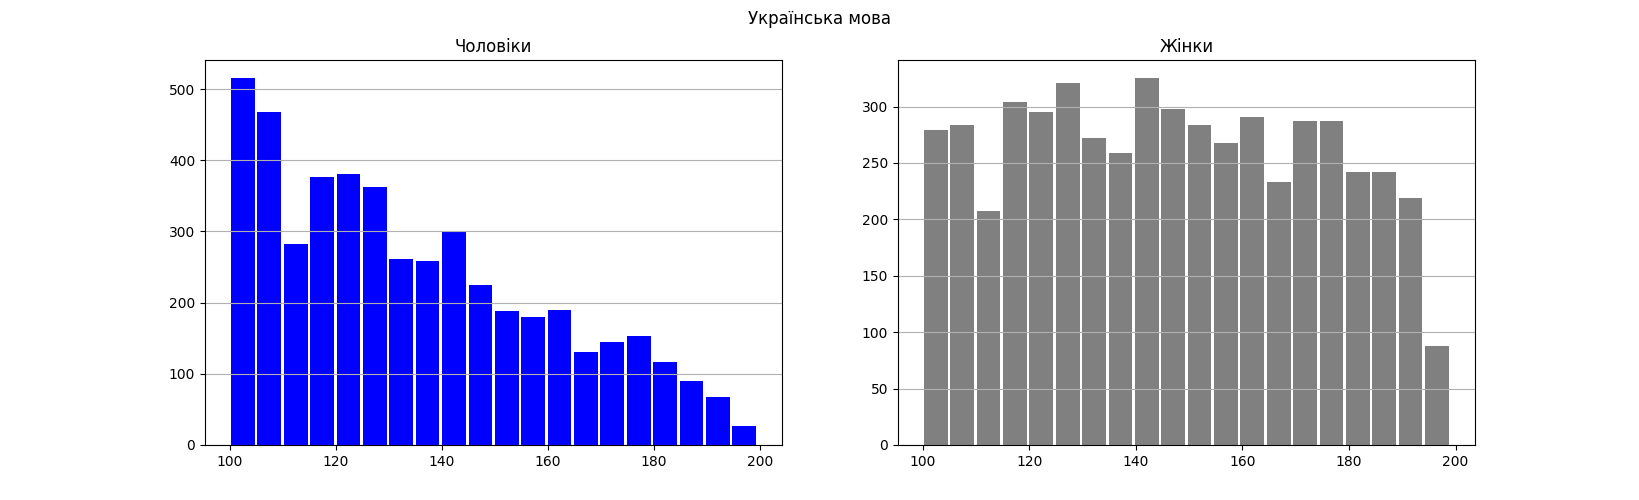
\includegraphics[trim=4cm 0cm 4cm 1cm, clip, width=1\linewidth]{UKR figures/UKR_10000.png}}
    \caption{Результати з української мови}
    \label{figure: UKR initial data}
\end{figure}

На малюнку наведено розподіл балів чоловіків та жінок: неозброєним оком бачимо наявну відмінність отриманих 
оцінок в залежності від статі. З'ясуємо, чи ця відмінність є статистично значущою.

\subsection{Перевірка гіпотези однорідності даних}

Нехай маємо дві незалежні вибірки $\left\{ X_i \right\}$ та $\left\{ Y_j \right\}$ однаково розподілених 
випадкових величин, розподіли $F_x$ й $F_y$ яких нам невідомі:
\begin{align*}
    &X_1 \ldots X_n\sim F_x && \text{результати чоловіків} \\
    &Y_1 \ldots Y_m\sim F_y && \text{результати жінок}
\end{align*}

Перевіримо гіпотезу про однорідність статистичного матеріалу, тобто гіпотезу, що ймовірності 
спостереження умовно високих, помірних та низьких балів в обох вибірках є однаковими. Таким чином 
матимемо $k=2$ вибірок, в яких елементи приймають $s=3$ різних значень. Для формалізації задачі 
введемо позначення:
\[ p_{ij}=\left\{
    \parbox[c]{13cm}{
    оцінка з чоловічо$\text{ї}_{(i=1)}$ чи жіночо$\text{ї}_{(i=2)}$ вибірки належить множині 
    високи$\text{х}_{(j=1)}$, помірни$\text{х}_{(j=2)}$ чи низьки$\text{х}_{(j=3)}$ балів
    } \right\} 
\]

Категорізація на множини оцінок того чи іншого рівня базувалася на прохідних балах на 
різні факультети КПІ у 2019 році (із переліком прохідних балів можна ознайомитися за 
\href{https://kpi.ua/2019-score}{посиланням}). 

При цьому <<високі>> оцінки обиралися із міркувань, що вступнику із таким балом доступно для 
вступу на бюджет більше ніж $65\%$ усіх факультетів, натомість абітурієнту із <<низькими>> 
оцінками рівень доступності значно нижчий -- лише $30\%$. До прикладу: 
\begin{align*}
    &A_1=\{ \text{оцінки, вищі за 178 балів} \} \\
    &A_2=\{ \text{оцінки між 144 та 178 балами} \} \\
    &A_3=\{ \text{оцінки, нижчі за 144 бали} \}
\end{align*}

Остаточно гіпотеза перевірки однорідності спосережуваних даних формулюватиметься так:
\begin{align}
    &\text{нульова гіпотеза} &&H_0: p_{11}=p_{21},\ p_{12}=p_{22},\ p_{13}=p_{23} \label{formula: hypothesis} \\
    &\text{проти альтернативи} && H_1: \exists i,j\quad p_{1,j}\neq p_{2,j} \nonumber
\end{align}

А тоді критерієм перевірки гіпотези слугуватиме правило
\begin{equation}
    \delta(x_1\ldots x_n,\ y_1\ldots y_m)=
    \begin{cases}
        H_1, & \rho\geqslant\chi^2_{1-\alpha;\ (k-1)(s-1)} \\
        H_0, & \rho<\chi^2_{1-\alpha;\ (k-1)(s-1)} \\
    \end{cases}\ , \label{formula: criterion}
\end{equation}

де статистика критерію $\rho$ обчислюється так:
\begin{equation}
    \rho\equiv \rho(x_1\ldots x_n,\ y_1\ldots y_m)=(n+m)\left( \sum\limits_{i=1}^k \sum\limits_{j=1}^s 
    \frac{\vartheta_{ij}^2}{\vartheta_{i\cdot}\vartheta_{\cdot j}} - 1\right), \label{formula: criterion statistics}
\end{equation}

величина критичної точки $\chi^2_{1-\alpha;\ (k-1)(s-1)}$ є квантилем рівня $(1-\alpha)$ розподілу Ст'юдента 
із $(k-1)(s-1)$ степенями свободи, а також
\begin{align*}
    &\vartheta_{1j}=\sum\limits_{i=1}^{n}\mathds{1}(X_i\in A_j) 
        && \parbox[c]{9.3cm}{частота потрапляння елементів вибірки \\ результатів чоловіків в одну із $j$ категорій} \\
    &\vartheta_{2j}=\sum\limits_{i=1}^{m}\mathds{1}(Y_i\in A_j) 
        && \parbox[c]{9cm}{частота потрапляння елементів вибірки \\ результатів жінок в одну із $j$ категорій} \\
    &\vartheta_{i\cdot}=\sum\limits_{j=1}^{s}\vartheta_{ij},\ \vartheta_{\cdot j}=\sum\limits_{i=1}^{k}\vartheta_{ij} 
        && \parbox[c]{9cm}{суми відповідних рядків чи стовпців \\ таблиці спостережуваних даних}
\end{align*}

\newpage
\subsubsection{Таблиця спостережуваних даних}

Складемо таблицю за спостережуваними даними навмання обраних $n=500$ та $m=500$ елементів із вибірок 
результатів ЗНО з української мови для чоловіків та жінок:

\begin{table}[H]
    \vspace*{0.8cm}
    \begin{center}
        \begin{tabular}{|c||c|c|c|c|}
            \hline
             & \text{Низькі бали} & \text{Помірні бали} & \text{Високі бали} & \text{Всього} \\
            \hline \hline
            \text{Чоловіки} & 343 & 125 & 32 & 500 \\
            \hline
            \text{Жінки} & 231 & 186 & 83 & 500 \\
            \hline
            \text{Всього} & 574 & 311 & 115 & 1000 \\
            \hline
        \end{tabular}
        \caption{Таблиця спостережуваних значень з української мови}
        \label{table: UKR homogeneity data}
    \end{center}
\end{table}

Обчислимо значення статистики критерію:
\begin{equation*}
    \rho = 1000\left( \frac{343^2}{574\cdot 500}+\frac{125^2}{311\cdot 500} + \ldots + 
    \frac{186^2}{311\cdot 500}+\frac{83^2}{115\cdot 500} - 1 \right) = 56.44
\end{equation*}

Водночас на рівні значущості $\alpha=0.01$ значення критичної точки
\begin{equation*} 
    \chi^2_{1-\alpha;\ (k-1)(s-1)}=\chi^2_{0.99;\ (2-1)(3-1)}=\chi^2_{0.99;\ 2}=9.21
\end{equation*}

\subsubsection{Висновок}

Оскільки значення статистики критерію перевищує значення критичної точки, то згідно критерію 
(\ref{formula: criterion}) гіпотеза про однорідність статистичних даних відхиляється. 
Отже, ймовірності спостереження оцінок різного рівня у вибірках для чоловіків та жінок, 
відповідно, різняться, тобто наявна ситуація неоднакового розполіду балів в залежності від статі.

\subsubsection*{Значення \texttt{p-value}}

Нехай випадкова величина $\tau$ має такий самий розподіл, як і статистика критерію й при цьому не залежить 
від неї: $\tau\sim\chi^2(2)$. Тоді величина \texttt{p-value} обчислюється як така ймовірність:
\[ P(\tau>\rho\ |\ H_0) = P(\tau>56.44) = 1-P(\tau\leqslant56.44) = 1-F_{\tau}(56.44) = 0.0001 \]

Тож при значенні $\alpha < \texttt{p-value}$ гіпотеза $H_0$ приймалася б.

\subsection{Нормалізація даних}

Як уже зазначалося, маємо дві незалежні вибірки $\left\{ X_i \right\}$ та $\left\{ Y_j \right\}$ 
однаково розподілених випадкових величин, розподіли $F_x$ й $F_y$ яких нам невідомі:
\begin{align*}
    &X_1 \ldots X_n\sim F_x && \text{результати чоловіків} \\
    &Y_1 \ldots Y_m\sim F_y && \text{результати жінок}
\end{align*}

Тим не менш, великий обсяг початкових даних дозволяє розбити оригінальні спостереження $\left\{ X_i \right\}$ й 
$\left\{ Y_j \right\}$ на значну кількість достатньо великих випадково сформованих неперетинних множин виду 
\[ \left\{ X^1_j \right\}_{j=\overline{1,n}}\ldots \left\{ X^N_j \right\}_{j=\overline{1,n}} \text{ й } 
   \left\{ Y^1_j \right\}_{j=\overline{1,n}}\ldots \left\{ Y^N_j \right\}_{j=\overline{1,n}}, \]

та надалі розглядати ці набори як незалежні дослідження. Причому в силу центральної граничної теореми 
(далі -- ЦГТ) із наявних наборів можна сформувати вибірки з $N$ величин, які мають нормальний розподіл:
\begin{align}
    &\overline{X^1}\ldots \overline{X^N}\sim N(\mu_x,\tfrac{1}{n}\sigma_x^2) && \text{середні результати чоловіків,} \label{formula: initail ND X} \\
    &\overline{Y^1}\ldots \overline{Y^N}\sim N(\mu_y,\tfrac{1}{n}\sigma_y^2) && \text{середні результати жінок,} \label{formula: initail ND Y}
\end{align}

де
\[ \overline{X^i}=\frac{1}{n}\sum\limits_{j=1}^nX^i_j,\ \overline{Y^i}=\frac{1}{n}\sum\limits_{j=1}^nY^i_j,\ i=\overline{1,N} \]

Схематично зобразимо суть процесу нормалізації початкових даних на прикладi вибірки $\left\{ X_i \right\}:$
\begin{equation}
    \begin{array}{lr}
        X^1_1 \ldots X^1_n\sim F_x \\
        \hfill{\ldots}\hfill \\
        X^N_1 \ldots X^N_n\sim F_x
    \end{array}
    \xRightarrow[]{\text{ ЦГТ }}
    \begin{array}{lr}
        \sqrt{n}\cdot \dfrac{\overline{X^1}-\mu_x}{\sqrt{\sigma_x^2}}\sim N(0,1) \\
        \hfill{\ldots}\hfill \\
        \sqrt{n}\cdot \dfrac{\overline{X^N}-\mu_x}{\sqrt{\sigma_x^2}}\sim N(0,1)
    \end{array} \label{formula: normalization scheme}
\end{equation}

Виконаємо ланцюжок нормалізації на прикладі вибірки результатів чоловіків. ЦГТ для достатньо великої 
фіксованої кількості $n$ випадково обраних елементів послідовності незалежних однаково розподілених 
випадкових величин матиме вид:
\begin{equation*}
    \frac{\sum\limits_{i=1}^nX_i-M\sum\limits_{i=1}^nX_i}{\sqrt{D\sum\limits_{i=1}^nX_i}}\approx N(0,1)
\end{equation*}

Спростимо вираз, використовуючи позначення $\mu_x=MX_i,\ \sigma_x^2=DX_i$ та скориставшись властивостями 
дисперсії та математичного сподівання:
\begin{equation*}
    \frac{n\overline{X}-n\mu_x}{\sqrt{n\sigma_x^2}}\approx N(0,1),\ \text{де}\ \overline{X}=\frac{1}{n}\sum\limits_{i=1}^nX_i
\end{equation*}

Залишивши $n$ виключно у знаменнику, матимемо:
\begin{equation*}
    \frac{n\overline{X}-n\mu_x}{\sqrt{n\sigma_x^2}}\approx N(0,1)\ \Rightarrow\ 
    \frac{\overline{X}-\mu_x}{\sqrt{\sigma_x^2/n}}\approx N(0,1)\ \Rightarrow\
    \overline{X}\approx N(\mu_x,\tfrac{1}{n}\sigma_x^2)
\end{equation*}

При розгляді такої ж кількості спостережень $n$ аналогічним чином отримуємо знормоване значення 
результатів жінок, де $\mu_y=MY_i,\ \sigma_y^2=DY_i:$
\begin{equation*}
    \overline{Y}\approx N(\mu_y,\tfrac{1}{n}\sigma_y^2)
\end{equation*}

Таким чином крок за кроком з початкових спостережуваних результатів утворюємо $N$ випадково сформованих 
неперетинних вибірок, вибіркові середні яких мають нормальний розподіл. Результат показано у виразах 
(\ref{formula: initail ND X})-(\ref{formula: initail ND Y}).

\subsection{Перевірка гіпотези рівності дисперсій}

Повертаючись до отриманих наборів (\ref{formula: initail ND X}) та (\ref{formula: initail ND Y}), переконаємося, 
що новоутворені вибірки справді мають нормальний розподіл. Для цього побудуємо гістограми, які за означенням 
є наближеннями істинних щільностей, а потім візуально проаналізуємо отримані криві:

\begin{figure}[H]
    \center{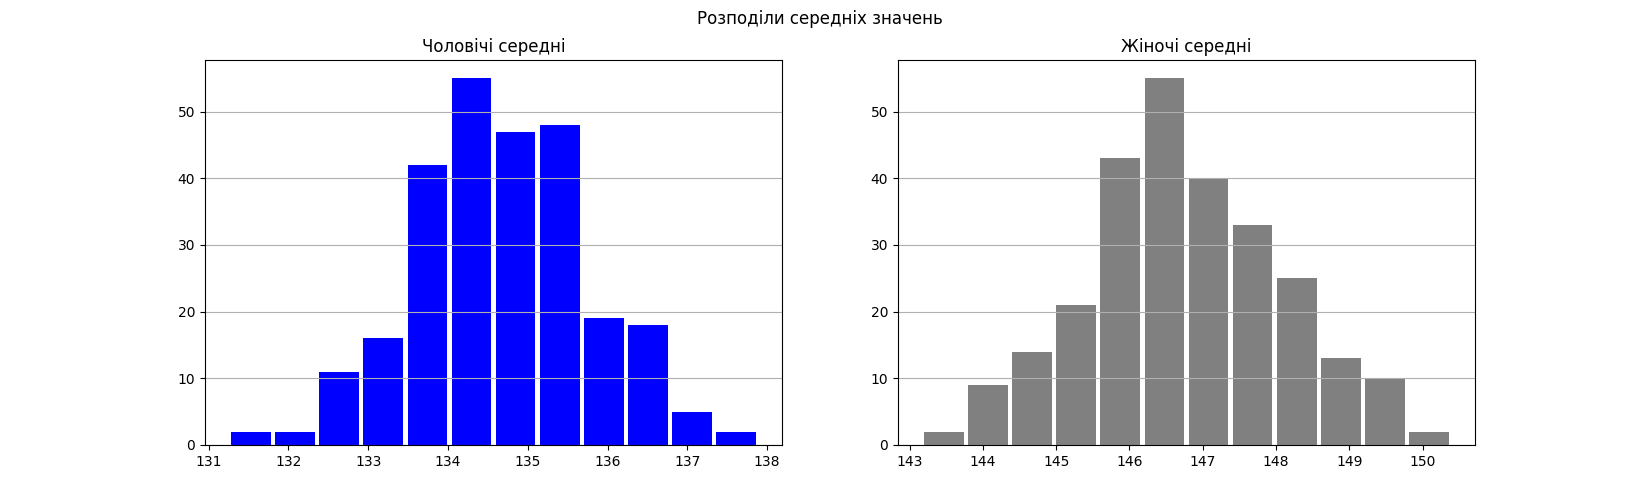
\includegraphics[trim=4cm 0cm 4cm 1cm, clip, width=1\linewidth]{UKR figures/Randomized_means_distribution_m500_N267_v8.png}}
    \caption{Гістограми наборів усереднених результатів ЗНО з української мови}
    \label{figure: UKR means data}
\end{figure}

Зауважимо, що криві в обох випадках мають схожі риси (мова про <<висоту>> та <<ширину>> графіків). 
Це дає підстави висунути й надалі первірити гіпотезу про рівність дисперсій вибірок результатів чоловіків 
та жінок.

\subsubsection{F-статистика Фішера}

Нехай задано дві незалежні нормально розподілені вибірки із невідомими параметрами: 
\begin{align*}
    &\overline{X^1}\ldots \overline{X^N}\sim N(\mu_x,\tfrac{1}{n}\sigma_x^2) && \text{середні результати чоловіків,} \\
    &\overline{Y^1}\ldots \overline{Y^N}\sim N(\mu_y,\tfrac{1}{n}\sigma_y^2) && \text{середні результати жінок,}
\end{align*}

при цьому
\[ \overline{X^i}=\frac{1}{n}\sum\limits_{j=1}^nX^i_j,\ 
   \overline{Y^i}=\frac{1}{n}\sum\limits_{j=1}^nY^i_j,\ i=\overline{1,N} \]

Перевіримо гіпотезу рівності невідомих дисперсій:
\begin{align*}
    &\text{нульова гіпотеза} && H_0: \sigma_x^2=\sigma_y^2 \\
    &\text{проти альтернативи} && H_1: \sigma_x^2\neq\sigma_y^2
\end{align*}

Або в еквівалентному записі:
\begin{align}
    &\text{нульова гіпотеза} && H_0:  \frac{\sigma_x^2}{\sigma_y^2}=1 \label{formula: F-test hypothesis} \\
    &\text{проти альтернативи} && H_1: \frac{\sigma_x^2}{\sigma_y^2}\neq 1 \nonumber
\end{align}

Скористаємося статистикою Фішера як статистикою критерію перевірки вищевказаної гіпотези. 
Перш за все зазначимо, що в силу нормальної розподіленості заданих вибірок нищевказані випадкові 
величини матимуть розподіл хі-квадрат із $(N-1)$ степенями свободи: 
\begin{equation} 
    \xi\equiv\frac{(N-1)S_X^2}{\sigma_x^2/n} \sim \chi^2(N-1),\ 
    \eta\equiv\frac{(N-1)S_Y^2}{\sigma_y^2/n} \sim \chi^2(N-1), \label{formula: F-test chi distributed}
\end{equation}

де значення
\begin{equation*}
    S_X^2=\frac{1}{N-1}\sum\limits_{i=1}^N(\overline{X^i}-\overline{X})\quad \text{та} \quad
    S_Y^2=\frac{1}{N-1}\sum\limits_{i=1}^N(\overline{Y^i}-\overline{Y})
\end{equation*}

є вибірковими дисперсіями двох наборів вибірок середніх результатів, а

\begin{equation*}
    \overline{X}=\frac{1}{N}\sum\limits_{i=1}^N \overline{X^i}\quad \text{й} \quad
    \overline{Y}=\frac{1}{N}\sum\limits_{i=1}^N \overline{Y^i}
\end{equation*}

є вибірковими середніми відповідних вибірок.

Оскільки обидві величини (\ref{formula: F-test chi distributed}) мають розподіл хі-квадрат та є незалежними, 
то випадкова величина
\begin{equation*}
    \zeta\overset{\mathrm{def}}{=}\frac{\eta/(N-1)}{\xi/(N-1)}\sim F\left( N-1,\ N-1 \right)
\end{equation*} 

має розподіл Фішера з $\left( N-1,\ N-1 \right)$ степенями свободи. Підставивши вирази 
(\ref{formula: F-test chi distributed}), матимемо:
\begin{equation*}
    \zeta=\frac{\sigma_x^2}{\sigma_y^2}\cdot \frac{S_Y^2}{S_X^2}\sim F\left( N-1,\ N-1 \right)
\end{equation*} 

При істиності нульової гіпотези $H_0: \frac{\sigma_x^2}{\sigma_y^2}=1$ отримаємо статистику критерію Фішера, 
яка визначатиметься так:
\begin{equation}
    \rho\equiv\rho(\overline{ x^1}\ldots \overline{x^N},\ \overline{y^1}\ldots \overline{y^N})=
    \frac{S_Y^2}{S_X^2}\sim F\left( N-1,\ N-1 \right) \label{formula: F-test statistic}
\end{equation}

Тоді перевищення чи недобір цією статистикою певних критичних значень формуватиме критичну область нульової 
гіпотези. Як наслідок критерієм перевірки гіпотези слугуватиме правило
\begin{equation}
    \delta\equiv\delta(\overline{ x^1}\ldots \overline{x^N},\ \overline{y^1}\ldots \overline{y^N})=
    \begin{cases}
        H_1, & \rho\leqslant k^* \text{ або } \rho\geqslant k^{**} \\
        H_0, & \rho\in (k^*,\ k^{**}) \\
    \end{cases}\ , \label{formula: F-test criterion}
\end{equation}

де значення критичних точок $k^*$ та $k^{**}$ при заданому рівні значущості $\alpha$ знайдемо з означення 
помилки першого роду: 
\begin{equation*}
    \alpha\overset{\mathrm{def}}{=}P(\delta\in K_{\alpha}\ |\ H_0)=
    P(\rho\leqslant k^* \text{ або } \rho\geqslant k^{**}\ |\ H_0)
\end{equation*}

Таким чином
\begin{equation*}
    \alpha=P(\rho\leqslant k^* \ |\ H_0) + P(\rho\geqslant k^{**}\ |\ H_0)
\end{equation*}

За умови однакової ймовірності цих подій матимемо:
\begin{equation}
    \begin{cases}
        P(\rho\leqslant k^* \ |\ H_0) = \frac{\alpha}{2} \\
        P(\rho\geqslant k^{**}\ |\ H_0) = \frac{\alpha}{2} \\
    \end{cases}
    \Rightarrow \
    \begin{cases}
        k^* = f_{\frac{\alpha}{2};\ (N-1,\ N-1)} \\
        k^{**} = f_{1-\frac{\alpha}{2};\ (N-1,\ N-1)} \\
    \end{cases}, \label{formula: F-test criterion values}
\end{equation}

де значення $k^*$ та $k^{**}$ є квантилями розподілу Фішера із $(N-1,\ N-1)$ степенями свободи при вказаному 
рівні значущості $\alpha$. Отже, за допомогою критичних точок~(\ref{formula: F-test criterion values})
та статистики критерію (\ref{formula: F-test statistic}) маємо змогу перевірити гіпотезу рівності дисперсій 
(\ref{formula: F-test hypothesis}) згідно критерія (\ref{formula: F-test criterion}).

\newpage
\subsubsection{Реалізація вибірки}

Розіб'ємо усю множину спостережуваних значень на $N=267$ неперетинних множин по $n=500$ елементів у кожній. 
У такому випадку статистична похибка обчислень є малою (детальніше -- на сторінці \pageref{page: UKR percentage point}). 
Наведемо потрібні величини для перевірки гіпотези рівності дисперсій у таблиці нижче:

\vspace{0.8cm}
\begin{table}[H]
    \begin{center}
        \begin{tabular}{||c|c|c|c|c|c||}
            \hline
            $n$ & $N$ & $\alpha$ & $S_X^2$ & $S_Y^2$ \\
            \hline \hline
            500 & 267 & 0.01 & 1.3501 & 1.6246 \\
            \hline
        \end{tabular}
        \caption{Значення шуканих параметрів F-тесту}
        \label{table: UKR F-test}
    \end{center}
\end{table}

Обчислимо значення статистики критерію:
\begin{equation*}
    \rho = \frac{S_Y^2}{S_X^2} = 1.2033
\end{equation*}

Водночас на рівні значущості $\alpha=0.01$ значення критичних точок
\begin{align*} 
   &k^* = f_{\frac{\alpha}{2};\ (N-1,\ N-1)} = f_{0.005;\ (266,\ 266)} = 0.7285 \\
   &k^{**} = f_{1-\frac{\alpha}{2};\ (N-1,\ N-1)} = f_{0.995;\ (266,\ 266)} = 1.3728
\end{align*}

\subsubsection{Висновок}
\label{page: UKR dispersion hypothesis}

Оскільки значення статистики критерію $\rho$ входить у проміжок $(0.7285,\ 1.3728)$, то згідно критерію 
(\ref{formula: F-test criterion}) на рівні значущості $\alpha=0.01$ нульова гіпотеза $H_0: \sigma_x^2=\sigma_y^2$ 
приймається. Для усіх подільших міркувань введемо таке позначення: $\sigma_x^2=\sigma_y^2=\sigma^2$.

\subsection*{Побудова довірчого інтервалу для різниці мат. сподівань}
\addcontentsline{toc}{subsection}{Побудова довірчого інтервалу для різниці математичних сподівань}

В результаті нормалізації початкових даних та перевірки гіпотези рівності дисперсій отримуємо такі дві вибірки: 
\begin{align}
    &\overline{X^1}\ldots \overline{X^N}\sim N(\mu_x,\tfrac{1}{n}\sigma^2) && \text{середні результати чоловіків,} \label{formula: UKR ND X} \\
    &\overline{Y^1}\ldots \overline{Y^N}\sim N(\mu_y,\tfrac{1}{n}\sigma^2) && \text{середні результати жінок,} \label{formula: UKR ND Y}
\end{align}

при цьому
\[ \overline{X^i}=\frac{1}{n}\sum\limits_{j=1}^nX^i_j,\ 
   \overline{Y^i}=\frac{1}{n}\sum\limits_{j=1}^nY^i_j,\ i=\overline{1,N} \]

Спробуємо оцінити, в якому інтервалі лежить значення різниці середніх балів для вибірок результатів ЗНО з 
української мови чоловіків та жінок.

\subsubsection{Пошук центральної статистики}
\label{page: seaching central statistic}

Перш за все віднайдемо для параметра $\theta=\mu_y-\mu_x$ центральну статистику 
\[ G \equiv G(\overline{X^1}\ldots \overline{X^N},\ \overline{Y^1}\ldots \overline{Y^N},\ \theta) \] 

Ця функція має задовільняти двом умовам: по-перше, її щільність розподілу $f_G(x)$ не залежить від параметра 
$\theta$, а по-друге, сама функція $G$ є неперервною і монотонною за $\theta$.
Виходячи з властивостей нормального розподiлу
\begin{equation*} 
    \overline{X}=\frac{1}{N}\sum\limits_{i=1}^N \overline{X^i} \sim N(\mu_x,\tfrac{1}{Nn}\sigma^2),\ 
    \overline{Y}=\frac{1}{N}\sum\limits_{i=1}^N \overline{Y^i} \sim N(\mu_y,\tfrac{1}{Nn}\sigma^2)
\end{equation*}

А отже, розподіл різниці $\overline{Y}-\overline{X}$ матиме вид
\[ \overline{Y}-\overline{X}\sim N(\mu_y-\mu_x,\ \tfrac{2}{Nn}\sigma^2) \]

Тоді позначимо
\begin{equation}
    \xi \equiv \frac{\overline{Y}-\overline{X}-(\mu_y-\mu_x)}{\sqrt{\tfrac{2}{Nn}\sigma^2}} \sim N(0,1) \label{formula: xi}
\end{equation}

В силу аналогічних до запису (\ref{formula: F-test chi distributed}) міркувань нищевказані випадкові 
величини матимуть розподіл хі-квадрат із $(N-1)$ степенями свободи: 
\begin{equation} 
    \frac{(N-1)S_X^2}{\sigma^2/n} \sim \chi^2(N-1),\ 
    \frac{(N-1)S_Y^2}{\sigma^2/n} \sim \chi^2(N-1), \label{formula: deviations}
\end{equation}

де
\begin{align*}
    &\begin{array}{lr}
        S_X^2=\frac{1}{N-1}\sum\limits_{i=1}^N(\overline{X^i}-\overline{X}) \\
        S_Y^2=\frac{1}{N-1}\sum\limits_{i=1}^N(\overline{Y^i}-\overline{Y})
    \end{array} &&
    \parbox[c]{7cm}{
        вибіркові дисперсії двох наборів вибірок середніх результатів
    }
\end{align*}

А отже, сума випадкових величин (\ref{formula: deviations}) як сума незалежних випадкових величин матиме 
розподіл $\chi^2$ із $\left[ (N-1)+(N-1) \right]$ степенями свободи:
\begin{equation}
    \eta \equiv \frac{(N-1)}{\sigma^2/n}\left( S_X^2+S_Y^2 \right)\sim \chi^2\left[ 2(N-1) \right] \label{formula: eta}
\end{equation}

Тоді випадкова величина
\begin{equation}
    \zeta \overset{\mathrm{def}}{=} \frac{\xi}{\sqrt{\frac{\eta}{2(N-1)}}} \sim t\left[ 2(N-1) \right] \label{formula: zeta}
\end{equation}

має розподіл Ст'юдента із $\left[ 2(N-1) \right]$ степенів свободи. Підставивши вирази (\ref{formula: xi}) й 
(\ref{formula: eta}) у формулу (\ref{formula: zeta}), отримаємо шукану центральну статистику для параметра 
$\theta=\mu_y-\mu_x:$
\begin{equation}
    G=\left((\overline{Y}-\overline{X})-\theta\right)\cdot 
    \sqrt{\frac{N}{S_X^2+S_Y^2}}
    \sim t\left[ 2(N-1) \right] \label{formula: G central statistic}
\end{equation}

\subsubsection{Виокремлення проміжку можливих значень параметра}

Побудуємо довірчий інтервал рівня довіри $\gamma:$
\begin{equation*}
    \gamma \overset{\mathrm{def}}{=}P(g_1<G<g_2)=\int\limits_{g_1}^{g_2}f_G(x)\ dx
\end{equation*}

В силу симетричності розподілу Ст'юдента, найкоротший центральний довірчий інтервал матиме вид:
\begin{equation}
    \gamma = P(g_1<G<g_2)=P(|\, G\, |<g) \label{formula: gamma t interval}
\end{equation}

На малюнку нижче схематично зображено ідею пошуку довірчого інтервалу та визначення відповідного 
квантиля $g:$ 

\begin{figure}[H]
    \center{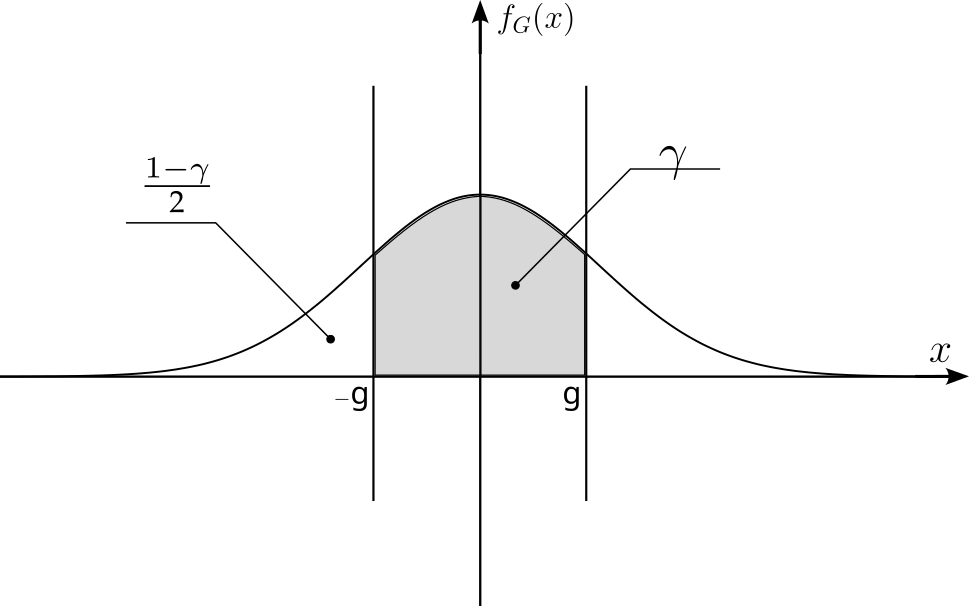
\includegraphics[width=0.9\linewidth]{UKR figures/t_confidence_interval.png}}
    \caption{Пошук квантиля розподілу Ст'юдента}
    \label{figure: t interval}
\end{figure}

Тож враховуючи, що 
$\int\limits_{-\infty}^{\infty}f_G(x)\ dx \overset{\mathrm{def}}{=} 1$, матимемо такий ланцюжок міркувань:
\begin{equation*}
    \int\limits_{-\infty}^{g}f_G(x)\ dx=\tfrac{1-\gamma}{2}+\gamma=\tfrac{1+\gamma}{2}\ \Rightarrow\
        F_t(g)= \tfrac{1+\gamma}{2}\ \Rightarrow\ 
        g = t_{\frac{1+\gamma}{2};\ 2(N-1)}
\end{equation*} 

Знайдено квантиль рівня $\frac{1+\gamma}{2}$ розподілу Ст'юдента із $\left[ 2(N-1) \right]$ степенями свободи. Підставляючи 
усі отримані результати у формулу (\ref{formula: gamma t interval}), отримаємо:
\begin{equation}
    \gamma = P\left( 
        -t_{\tfrac{1+\gamma}{2};\ 2(N-1)} < 
        \left((\overline{Y}-\overline{X})-\theta\right)\cdot \sqrt{\frac{N}{S_X^2+S_Y^2}} < 
        t_{\tfrac{1+\gamma}{2};\ 2(N-1)} 
    \right) \label{formula: UKR t trusted interval}
\end{equation}

\subsubsection{Реалізація вибірки}

Останнім кроком вкажемо конкретні значення усіх необхідних величин:

\vspace{0.8cm}
\begin{table}[H]
    \begin{center}
        \begin{tabular}{||c|c|c|c|c|c|c||}
            \hline
            $n$ & $N$ & $\gamma$ & $g=t_{0.975;\ 532}$ & $S_X^2$ & $S_Y^2$ & $\overline{Y}-\overline{X}$ \\
            \hline \hline
            500 & 267 & 0.95 & 1.96 & 1.3501 & 1.6246 & 12.0768 \\
            \hline
        \end{tabular}
        \caption{Значення параметрів для довірчого інтервалу різниці середніх}
        \label{table: UKR t interval}
    \end{center}
\end{table}

Підставивши у вираз (\ref{formula: UKR t trusted interval}) значення, які наведені у таблиці вище, отримаємо 
такий довірчий інтервал для параметра $\theta=\mu_y-\mu_x$:
\begin{equation*}
    P(11.87 < \theta < 12.28)=0.95
\end{equation*}

\subsubsection{Висновок}

Отримано довірчий інтервал рівня довіри $\gamma=0.95$ для величини різниці середніх значень 
оцінок з української мови вибірок результатів чоловіків та жінок: $(11.87,\ 12.27)\ni \mu_y-\mu_x$. Оскільки 
у вказаному проміжку немає нульового значення, гіпотезу про нерозрізнюваність середніх можна відхилити. 

Можемо стверджувати, що при порівнянні результатів чоловіка та жінки оцінка з української мови у жінки буде 
більшою за оцінку у чоловіка на бал у $12.08\pm 0.2$ пункти, при цьому в середньому у п'яти зі ста таких 
порівнянь вказане наближення може бути хибним.

\subsection{Побудова довірчого інтервалу для значення дисперсії}

Наступним кроком віднайдемо проміжок можливих значень дисперсії, або інакше кажучи, розсіяння навколо 
математичного сподівання нормованих вибірок. В силу прийняття гіпотези рівності дисперсій 
(сторінка \pageref{page: UKR dispersion hypothesis}) із оригінальних наборів
\begin{align*}
    &\overline{X^1}\ldots \overline{X^N}\sim N(\mu_x,\tfrac{1}{n}\sigma^2) && \text{середні результати чоловіків} \\
    &\overline{Y^1}\ldots \overline{Y^N}\sim N(\mu_y,\tfrac{1}{n}\sigma^2) && \text{середні результати жінок}
\end{align*}

аналогічними кроками (як на сторінці \pageref{page: seaching central statistic}) можна сформувати випадкову 
величину (\ref{formula: eta}) розподілу хі-квадрат із $\left[ 2(N-1) \right]$ степенями свободи, при цьому 
для параметра дисперсії $\frac{1}{n}\sigma^2$ ця величина відіграватиме роль центральної статистики:
\begin{equation}
    G\equiv\frac{(N-1)}{\sigma^2/n}\left( S_X^2+S_Y^2 \right)\sim \chi^2\left[ 2(N-1) \right]
\end{equation}

А тоді довірчий інтервал рівня довіри $\gamma$ матиме вид:
\begin{equation}
    \gamma \overset{\mathrm{def}}{=} P(g_1<G<g_2)=\int\limits_{g_1}^{g_2}f_G(x)\ dx \label{formula: gamma chi interval}
\end{equation}

На рисунку нижче схематично показано пошук величин $g_1$ та $g_2:$

\begin{figure}[H]
    \vspace{0.3cm}
    \center{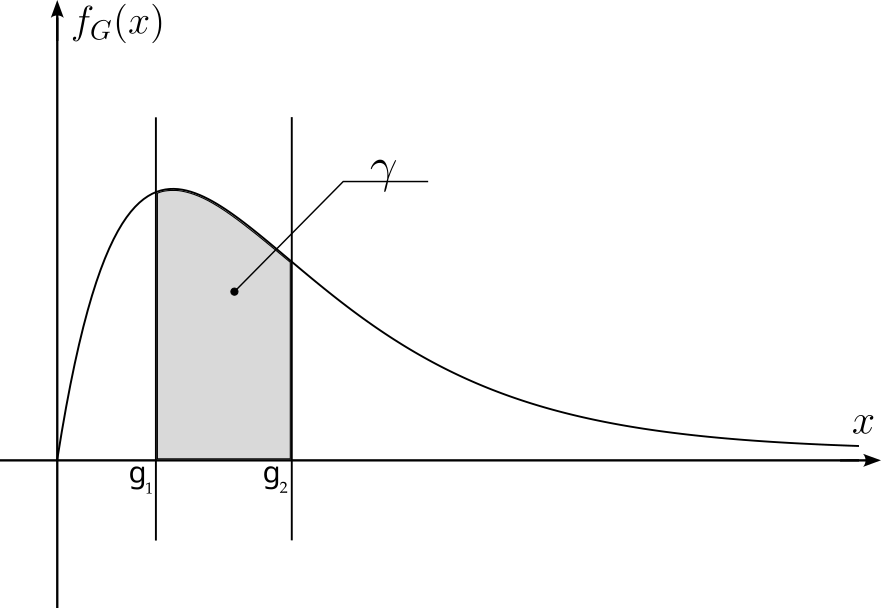
\includegraphics[width=0.8\linewidth]{UKR figures/chi_confidence_interval.png}}
    \caption{Пошук квантилів розподілу хі-квадрат}
    \label{figure: chi interval}
\end{figure}

Тож значення $g_1$ та $g_2$ є квантилями рівнів $\frac{1-\gamma}{2}$ та $\frac{1+\gamma}{2}$ розподілу 
хі-квадрат із $\left[ 2(N-1) \right]$ степенями свободи:
\begin{align*}
    &\int\limits_{0}^{g_1}f_G(x)\ dx=\tfrac{1-\gamma}{2}\ \Rightarrow\ 
        F_{\chi^2}(g_1)=\tfrac{1-\gamma}{2}\ \Rightarrow\
        g_1=\chi^2_{\tfrac{1-\gamma}{2};\ 2(N-1)} \\
    &\int\limits_{0}^{g_2}f_G(x)\ dx=\tfrac{1+\gamma}{2}\ \Rightarrow\ 
        F_{\chi^2}(g_2)=\tfrac{1+\gamma}{2}\ \Rightarrow\
        g_2=\chi^2_{\tfrac{1+\gamma}{2};\ 2(N-1)}
\end{align*}

Підставляючи отримані результати у формулу (\ref{formula: gamma chi interval}), отримаємо:
\begin{equation}
    \gamma = P\left( 
        \chi^2_{\tfrac{1-\gamma}{2};\ 2(N-1)} < 
        \frac{(N-1)}{\sigma^2/n}\left( S_X^2+S_Y^2 \right) < 
        \chi^2_{\tfrac{1+\gamma}{2};\ 2(N-1)} 
    \right) \label{formula: UKR chi trusted interval}
\end{equation}

\newpage
Наостанок вкажемо конкретні значення усіх необхідних величин:

\vspace{0.8cm}
\begin{table}[H]
    \begin{center}
        \begin{tabular}{||c|c|c|c|c|c|c||}
            \hline
            $n$ & $N$ & $\gamma$ & $g_1=\chi^2_{0.025;\ 532}$ & $g_2=\chi^2_{0.975;\ 532}$ & $S_X^2$ & $S_Y^2$ \\
            \hline \hline
            500 & 267 & 0.95 & 469.98 & 597.80 & 1.3501 & 1.6246 \\
            \hline
        \end{tabular}
        \caption{Значення параметрів для довірчого інтервалу дисперсії}
        \label{table: UKR chi interval}
    \end{center}
\end{table}

Підставивши у вираз (\ref{formula: UKR chi trusted interval}) наведені вище значення, отримаємо 
такий довірчий інтервал для параметра $\frac{1}{n}\sigma^2:$
\begin{equation*}
    P(1.32\ < \frac{\sigma^2}{n} <\ 1.68)=0.95
\end{equation*}

\subsubsection{Висновок}

Таким чином для сформованих нормально розподілених вибірок (\ref{formula: UKR ND X})-(\ref{formula: UKR ND Y}) 
значення дисперсії в середньому лише у п'яти елементів вибірки зі ста буде виходити за межі проміжку від $1.32$ 
до $1.68$ балів.

\subsection{Статистична похибка обчислень}
\label{page: UKR percentage point}

Статистичною похибкою обчислень називатимемо найменшу величину $\Delta$ відхилення різниці вибіркових 
середніх від істинного значення різниці математичних сподівань заданих вибірок (\ref{formula: UKR ND X})-(\ref{formula: UKR ND Y}) 
з щонайменшою ймовірністю у $95\%$. Тобто шукана похибка $\Delta$ обчислюватиметься як така ймовірність:
\begin{equation*}
    P\left(\ \left| (\overline{Y}-\overline{X})-(\mu_y-\mu_x) \right| \leqslant \Delta\ \right)\geqslant 0.95
\end{equation*}

Домножимо обидві частини нерівності всередині аргументу ймовірності на певну величину:
\begin{equation*}
    P\left(\ \underbracket{\left| (\overline{Y}-\overline{X})-(\mu_y-\mu_x) \right| \cdot \sqrt{\frac{N}{S_X^2+S_Y^2}}} 
    \leqslant \Delta \cdot \sqrt{\frac{N}{S_X^2+S_Y^2}} \ \right)\geqslant 0.95
\end{equation*}

Після розкриття модуля та в ході аналогічних міркувань, які наведені для заданих вибірок на сторінці 
\pageref{page: seaching central statistic}, з формули (\ref{formula: G central statistic}) випливає, що 
випадкова величина в лівій частини нерівності має розподіл Ст'юдента з $\left[ 2(N-1) \right]$ степенями 
свободи. А відтак шукана ймовірність згідно означення функції розподілу виглядатиме так:
\begin{equation*}
    2F_t\left( \Delta \cdot \sqrt{\frac{N}{S_X^2+S_Y^2}} \right)-1 \geqslant 0.95
\end{equation*}

У такому разі величина похибки $\Delta$ виражатиметься через квантиль рівня $0.975$ розподілу Ст'юдента з 
$\left[ 2(N-1) \right]$ степенями свободи:
\begin{equation}
    \Delta \geqslant t_{0.975;\ 2(N-1)} \cdot \sqrt{\frac{S_X^2+S_Y^2}{N}} \label{formula: percentage point}
\end{equation}

Таблиця необхідних значень виглядатиме таким чином:

\vspace{0.8cm}
\begin{table}[H]
    \begin{center}
        \begin{tabular}{||c|c|c|c||}
            \hline
            $N$ & $t_{0.975;\ 532}$ & $S_X^2$ & $S_Y^2$ \\
            \hline \hline
            267 & 1.96 & 1.3501 & 1.6246 \\
            \hline
        \end{tabular}
        \caption{Значення параметрів для обчислення статистичної похибки}
        \label{table: UKR percentage point}
    \end{center}
\end{table}

Тож остаточно найменша величина відхилення $\Delta = 0.21$, а тоді початкова ймовірнісна нерівність матиме вид:
\begin{equation*}
    P\left(\ \left| (\overline{Y}-\overline{X})-(\mu_y-\mu_x) \right| \leqslant 0.21\ \right)\geqslant 0.95
\end{equation*}

\subsubsection{Висновок}

Для встановлених значень $n=500$ й відповідно $N=267$ статистична похибка відхилення різниці вибіркових 
середніх від істинного значення різниці математичних сподівань складає $\Delta = 0.21$ бала з ймовірністю, 
більшою за $95\%$. Можемо стверджувати, що обчислення за такого значення похибки мають високу точність, 
оскільки величина $\Delta = 0.21$ є лише $0.1\%$ від можливих $200$ балів за результат тесту.